\section{Introdução}

Nesse capítulo fazemos uma revisão bibliográfica da área de Dinâmicas de
Opinião\footnote{Doravante OD (\textit{Opinion Dynamics}).} Definimos a área, o
que são modelos baseados em agente e quais os constituintes típicos de um modelo
de OD. Depois apresentamos modelos que podem ser considerados canônicos, em sua
versão mais simples, pelo fato de inspirarem uma gama de modificações e
extensões. Na seção seguinte discutimos algumas questões teóricas referentes à
atualização da opinião dos agentes e concluímos o capítulo com uma discussão de
nossa abordagem.


\section{Definição da Área}

OD é uma área que pode ser definida a partir de 3 elementos: primeiramente,
sistemas alvo em comum, delimitados pela pergunta central: quais elementos
determinam se um grupo de agentes chega ao consenso sobre algo, ou ao invés
disso persistem em discórdia? \cite{castellano2012social}\footnote{Essa pode ser
  pensada como a pergunta \textit{fundacional} da área \cite{flache2017}.} ;
segundo, um conjunto de modelos que partilham elementos constitutivos,
particularmente fazendo uso da técnica da Modelagem Baseada em
Agentes\footnote{De agora em diante vamos usar a abreviação ABM para modelagem
  (ou modelo(s)) baseada(os) em agentes.}, e em, alguma medida, de
\textit{insights} e técnicas da Física Estatística \cite{galam1990social};
terceiro, uma comunidade de pesquisadores que partilham do interesse no objeto,
fazem uso de referenciais e técnicas compartilhadas e se reconhecem como membros
dessa comunidade.

Na área há a aceitação de um significado amplo e abstrato de opinião como uma
característica de um agente que pode ser mudada com pouco custo
\cite[p.312]{castellano2012social}. Isso permite com que ela vise sistemas alvos
tais como voto, ciência, cultura, difusão de tarifas, dentre outros
\cite{kowalska2013going,martins2015thou,axelrod1997dissemination,galam1990social}.
Essa gama de aplicações está relacionada com a base disciplinar dos pesquisadores,
envolvendo pessoas de áreas como Física, Sociologia, Ciência Política, Economia,
Psicologia Social, dentre outras, o que nos permite considerar a área como um
subgrupo da Sociofísica \cite{galam1982sociophysics,galam2012sociophysics}.


\section{Modelagem Baseada em Agentes e Dinâmicas de Opinião}

Modelos Baseados em Agentes podem ser definidos como modelos que envolvem
agentes discretos, onde agentes, seus atributos, e possivelmente um ambiente são
definidos algoritmicamente \cite{sayama2015introduction} \footnote{ ABMs
  costumam ser implementados como simulações num computador, embora existam
  modelos baseados em agentes que historicamente não tenham sido diretamente em
  computadores, como os modelos de Schelling e de Sakoda
  \cite{hegselmann2017thomas}.}. Num ABM existem três noções primitivas: os
\textit{atributos}, os \textit{estados} e as \textit{configurações}
\cite[p.7]{de2014agent}. Os atributos dos agentes são o conjunto de propriedades
que cada cada agente \(i\) tem. Os estados dos agentes são os valores de seus
atributos num determinado tempo \(t\). Já as configurações são as coleções de
todos os estados dos agentes num modelo.

ABMs é uma técnica flexível: podemos construir modelos ``metafóricos'' com
objetivo de auxiliar o desenvolvimento de intuição segundo a elucidação de
princípios; ou de alta-fidelidade, com dezenas de atributos e um
ambiente incluindo casas, escolas, sistemas de transporte, dentre outros, com o
objetivo avaliar contrafactuais próximos a determinados casos concretos
\cite{de2014agent, epstein2006generative}.


Segundo \citeonline[p.430-1]{sayama2015introduction}, ABMs têm as seguintes
propriedades típicas:
\begin{itemize}
\item agentes podem ter estados internos;
\item agentes podem ser espacialmente localizados;
\item agentes podem perceber e interagir com o ambiente;
\item agentes podem interagir segundo regras pré-definidas;
\item agentes podem ser capazes de aprender e adaptar-se;
\item agentes podem interagir com outros agentes;
\item AMBs muitas vezes não tem supervisores/controladores centrais;
  \item ABMs podem produzir comportamentos coletivos não triviais.
  \end{itemize}

  Tendo em vista essas propriedades, ABMs são particularmente úteis para o
  estudo de sistemas complexos \cite{wilensky2015introduction}, dada: sua
  capacidade de incluir redes e espaço; seu potencial de ligar múltiplos
  domínios e de incluir uma maior heterogeneidade de agentes; além de seu foco
  na robustez de resultados \cite{de2014agent,wilensky2015introduction}. Não por
  acaso, ABMs são amplamente usados em OD  \cite{castellano2012social,flache2017}.

  Que elementos constituem os modelos de OD ? Podemos delimitar um modelo de
  dinâmicas de opinião da seguinte forma: agentes,conectados, possuem opiniões
  como variáveis e interagem segundo regras que explicam a mudança ou manutenção
  das opiniões individuais sob efeito da interação com outros agentes ou outras
  fontes (como a mídia) \cite{sirbu2017opinion}. Os agentes num modelo em OD tem
  então : uma \textit{opinião}; uma \textit{estrutura de interação}; e uma
  \textit{regra de atualização} de sua opinião.


  A opinião dos agentes pode ser representada como uma variável ou conjunto de
  variáveis, que por sua vez podem ser discretas ou contínuas. Já a estrutura de
  interação consiste no conjunto de agentes cujas ações e propriedades podem
  afetar a opinião de um agente \(i\) \cite{page2008uncertainty}.

  Podemos dividir a estrutura de interação numa \textit{topologia} de interação e
  numa \textit{regra de interação}. A topologia de interação define quais
  agentes estão conectados com \(i\), e podem, potencialmente, afetá-lo. A regra
  de interação define como \(i\) interage com os agentes desse conjunto(seus
  ``vizinhos''). Em OD as regras de interação definem qual a
  relação que o agente \(i\) tem com seus vizinhos: se interage com um vizinho
  por vez, uma interação em díade, ou com algum subconjunto de seus vizinhos,
  uma interação em grupo. Por fim, a regra de atualização define sob qual regra
  a opinião do agente \(i\) muda do tempo \(t\) para o tempo \(t+1\). 

  

  \section{Modelos Canônicos}

  Adaptações do Modelo de Ising são os modelos mais fundamentais na área. O
  modelo de Ising é um modelo paradigmático da Mecânica Estatística, usado para
  representar o processo de magnetização de materiais\footnote{O modelo de Ising
    é um modelo paradigmático de sistemas com muitas partes interagindo levando
    à uma transição de fase, a uma mudança de comportamento qualitativo do
    sistema. Sendo assim, é aplicado em vários contextos além da sua concepção
    original, como mercados financeiros, sistemas ecológicos, e dinâmicas de
    opinião \cite{sole2011phase}}. Neles, variáveis discretas, \textit{spins},
  com valores $s = \pm 1$, estão localizadas num grafo, e têm uma tendência a
  alinhar-se com seus vizinhos: se a maioria tem \(s = + 1 \) o spin muda seu
  valor para \(+1\); se a maioria tem \(s = -1 \) o spin muda seu valor para
  \(-1\); se houver empate o spin muda seu valor com probabilidade
  \(\frac{1}{2}\) \cite{castellano2012social,sole2011phase}. A reinterpretação
  para o contexto de OD é o seguinte: o spin é um agente; sua opinião pode ter
  os valores \(+1\) ou \(-1\); um agente interage com todos seus vizinhos por
  passo de tempo; ele assume a opinião da maioria deles.

  Um modelo parecido com o anterior é o ``Voter'' \cite{holley1975ergodic}. Nele
  cada agente tem uma opinião binária \(\pm\) 1 ; e a cada passo um agente é
  selecionado aleatoriamente e assume a opinião de algum de seus vizinhos.
  Difere do modelo anterior, portanto, na regra de interação, díade ao invés do
  grupo inteiro, e de atualização, assume o valor do vizinho ao invés da maioria
  deles.


  Já no modelo da Regra de Maioria de Serge Galam a interação é : a cada
  ``tick'' um grupo de tamanho \textit{r} é selecionado aleatoriamente e todos
  os agentes mudam sua opinião para a opinião da maioria do grupo
  \cite{galam1990social,galam2012sociophysics}. O tamanho \textit{r} pode ser
  fixo ou ser tirado de alguma distribuição a cada passo. Se \textit{r} for par
  podem ocorrer empates nos grupos, de forma que ou o grupo escolhe uma das
  opiniões com probabilidade \(\frac{1}{2}\), ou introduz-se um viés, e toda vez
  que houver empate o grupo muda para uma das opiniões
  \cite{galam2012sociophysics, galam1986majority}.

  Outro modelo bastante discutido na literatura é o Modelo Sznajd
  \cite{sznajd2000opinion}. Nele cada agente têm exatamente dois vizinhos, é uma
  grade unidimensional. A cada passo um par $ij$ de vizinhos é selecionado e se
  sua opinião for igual os outros vizinhos de \(i\) e \(j\) mudam a opinião para
  a opinião de convergência. Se eles discordarem, \(i\) adota a opinião do outro
  vizinho, e \(j\) faz o mesmo.

  
  Todos os modelos até agora representaram opiniões como uma variável que pode
  tomar valores binários. Além disso, com exceção do modelo Sznajd, a regra de
  atualização dos modelos pressupõe uma interação assimilativa: os agentes
  agentes assumem a opinião dos outros \cite{flache2017}. O modelo de
  \cite{axelrod1997dissemination} difere em ambos os aspectos. Baseia-se em dois
  princípios: a preferência dos indivíduos em interagir com pessoas similares
  (homofilia) e o aumento de similaridade após a interação (influência social).
  Cada agente tem por opinião um conjunto $F$ de variáveis $(\sigma_1 , \ldots, \sigma_f)$.
  Esses $\sigma_i$ podem tomar valores $q$ de 0 a $q-1$. As variáveis são chamadas de
  ``cultural features'' e seus possíveis valores de ``traits per feature''. O
  modelo considera interação entre pares de agentes, como o modelo voter, os
  quais só interagem se existerem ``traits'' iguais. Isso significa que a
  interação só é possível para indivíduos similares e acaba por torná-los mais
  similares.


\subsection{Modelos Contínuos}



\quad \quad Um dos modelos mais citados em OD é o modelo de
\citeonline{deffuant2000mixing}..
Nele a opinião é uma variável contínua que pode tomar valores de -1 a 1, $x_i \in
[-1,1]$. Dois agentes são escolhidos aleatoriamente e interagem se suas opiniões
forem próximas o bastante, onde próximo é um parâmetro de ``confiança'' ``d''.
Se eles interagirem suas opiniões se aproximam de acordo com um parâmetro $\mu$ :
$x_i = x_i + \mu(x_j - x_i)$. A população converge para um determinado ``cluster''
dependendo do parâmetro $d$. O parâmetro $\mu$ e o tamanho da população determinam
a velocidade de convergência e a largura da distribuição final de opiniões.

Outro modelo importante com agentes que tem uma opinião contínua é o modelo de
Hegselmann-Krause. Nesse modelo a regra de interação, e de atualização, difere
do modelo de Deffuant por ser social: os agentes interagem com todos os vizinhos
compatíveis,dado um parâmetro de confiança, ao mesmo tempo, e toma a média das
opiniões dos agentes vizinhos.


\section{Regra de Atualização e Processamento de Informação}


\quad \quad Nós temos o CODA\cite{martins2008continuous}\footnote{\textit{Continuous
    opinions and discrete actions}.}.Uma contribuição do modelo é exatamente em
deixar claro o papel da regra de atualização em separado à da interação. Agentes
observam opiniões discretas de outros agentes, e mudam sua opinião contínua
$p_i$ sobre essa opção a depender dos outros agentes. Esse $p_i$ quantifica a
adesão a uma opinião. E é atualizado por meio de atualização bayesiana. O modelo
é aplicado para regras de interação tanto voter ( $x_i $ versus $x_j$) quanto ao
sznajd, e em ambos ocorre a emergência de ``clusters'' de extremismo. \todo{Eu
  vou discutir mais o CODA!!!}

\begin{figure}[H]
  \centering 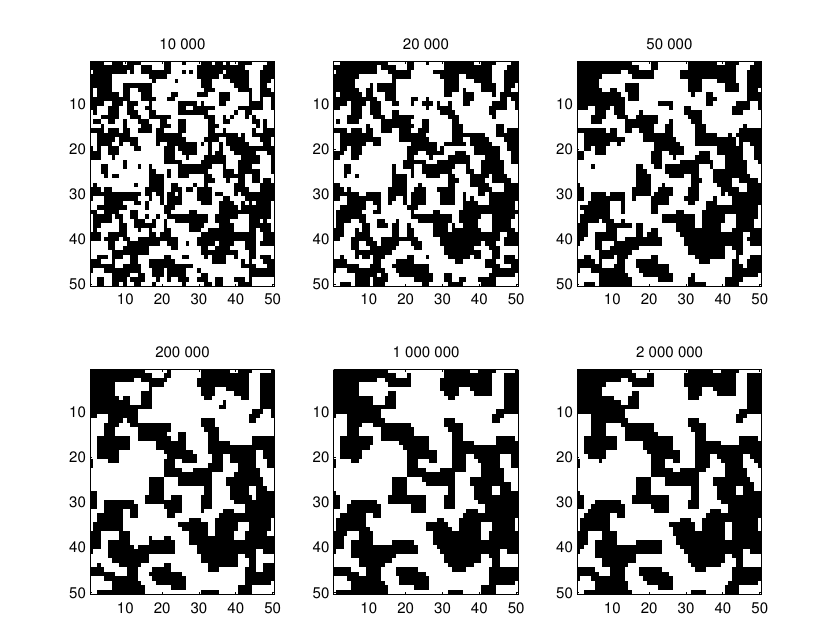
\includegraphics[scale = 0.7]{ims/andre.png}
  \caption{Evolução temporal do modelo CODA numa grade 50 x 50 com
    interação entre pares $ij$ (voter)}
  Fonte: \citeonline{martins2008continuous}
\end{figure}


Qual a razão intuitiva do CODA?  Quando alguém fica face uma escolha
binária, ou mais em geral discreta, sua opinião sobre qual a melhor
não é necessariamente discreta: a pessoa pode \textbf{crer} que uma
das alternativas é melhor com probabilidade p. Cada agente observa as
escolhas de outros indivíduos, mas não observa a opinião interna
deles, que é uma função de probabilidade contínua. Nós podemos pensar
que existem dois campos, o campo visível das ``ações'' e o campo por
detrás das opiniões \cite{martins2008continuous}.

 \citeonline{martins2012bayesian} oferece o seguinte passo a passo
para a construção de um modelo de dinâmicas de opinião no qual a opinião dos
agentes é uma função de probabilidade:

\begin{enumerate}
\item Identificar uma questão sob debate e chamá-la de $x$ . Uma
  escolha sobre diferentes ideais ou teorias é uma escolha discreta
  logo $x$ deve ser discreta. Se o debate for sobre uma variável
  contínua então $x$ é contínua.
\item cada agente tem uma opinião subjetiva sobre $x$ essa opinião é
  representada pela distribuição de probabilidade $f_i(x)$ .
\item Ocorre comunicação : a comunicação é a declaração de um valor
  $ A_j$ pelo agente $j$ de tal forma que $A_j[f]$ é um funcional de
  $f_j(x)$.
\item Os agentes tem que ter em sua mente  uma relação entre o
  verdadeiro valor entre $x$ e o valor declarado $A_j$. Isso é dado
  pela distribuição de probabilidade $P(A_j|x)$.
\item Dado o prior $f_i(x)$ a opinião posterior $f_i(x|A_j)$ é dada
  por $A_i[f_i(x|A_j)]$ que é a nova opinião de $i$ .
\end{enumerate}
